% !TeX spellcheck = en_US
\clearpage
\section{Experimental Setup}
The experimental setup consists of the following components:
\begin{itemize}
	\item Radiation source
	\item Semiconductor detector
	\item Vacuum container with pressure gauge, \\inlet (to let the air in) and outlet (for vacuum) valves
	\item Vacuum pump
	\item Preamplifier and main amplifier
	\item Power supply unit with external voltage measuring device
	\item Multi-channel pulse height analyzer (MCA) inside the PC
	\item PC with MCA software
\end{itemize}

Figure \ref{fig:aufbauhalbleiter} shows the experimental setup schematically, while photographs of the actual experiment are shown in Figure \ref{fig:setup_}. The surface barrier counter and the alpha radiation source are located in an airtight metal cylinder. The source can be moved in the cylinder along one spatial axis in order to change the distance between the source and detector. At the minimum adjustable distance, the source does not touch the detector. In fact, determining this minimum distance is part of the experiment.
\begin{figure}[h]
	\centering
	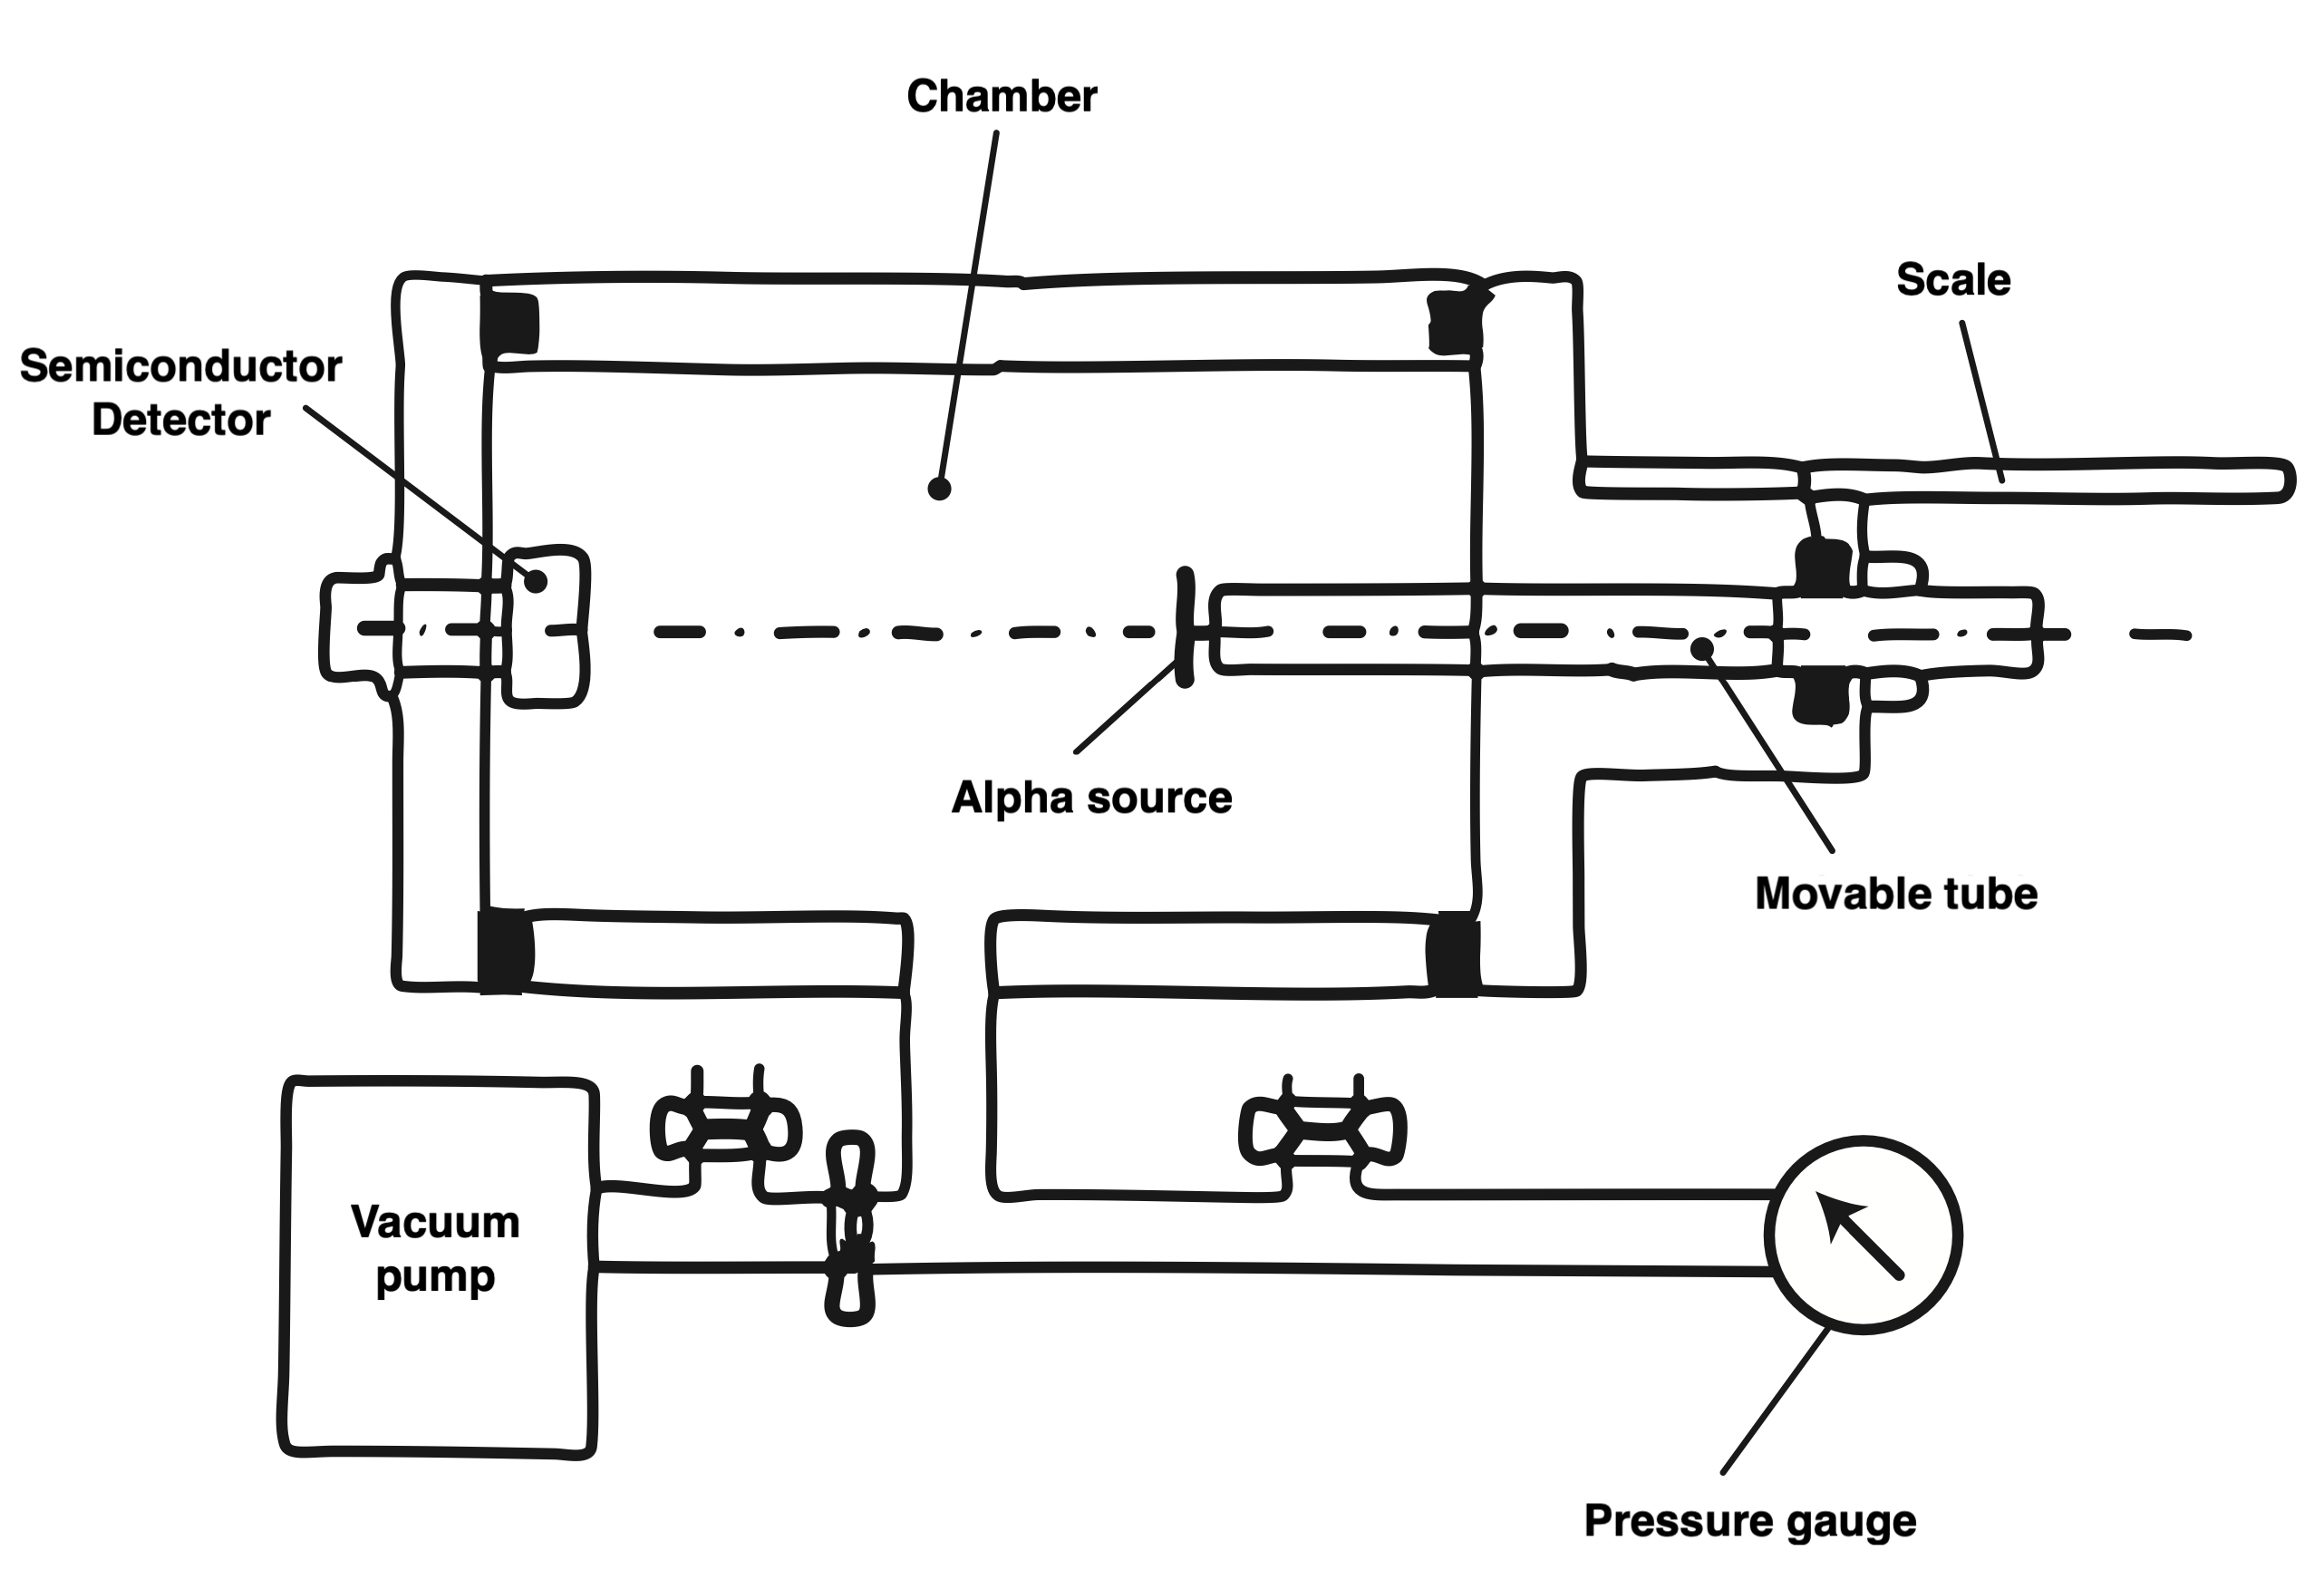
\includegraphics[width=0.7\linewidth]{img/schematics_exp.png}
	\caption{Schematics of the experimental setup.}
	\label{fig:aufbauhalbleiter}
\end{figure}

\hfill

The mixed source has an active area with a diameter of about 7~mm and is covered by a gold  layer, which is about 2~\textmu m thick (see Figure \ref{fig:quellefoto}). However, the covering of the radioactive material does not provide protection against contamination on contact. Hence, the source must be considered open and special licensing requirements and precautions must be taken into account (see section \ref{sec:warningnotices}).
The preamplifier is attached to the semiconductor detector directly outside the vacuum container. The entrance window of the detector can be seen in Figure \ref{fig:detektorfoto}. The preamplifier has several connections: 
\begin{itemize}[itemsep=0pt]
	\item Operating voltage supply, connected to the rear of the main amplifier.
	\item Signal output, connected to signal input of the main amplifier.
	\item External voltage input, connected to the power supply unit.
	\item Connection option for a pulser. Not connected.
\end{itemize}
The wiring of the experiment is shown in figure \ref{fig:verkabelung} and figure \ref{fig:setup3} shows a picture of the main amplifier as well as the voltage supply unit.
\begin{figure}[h]
	\centering
	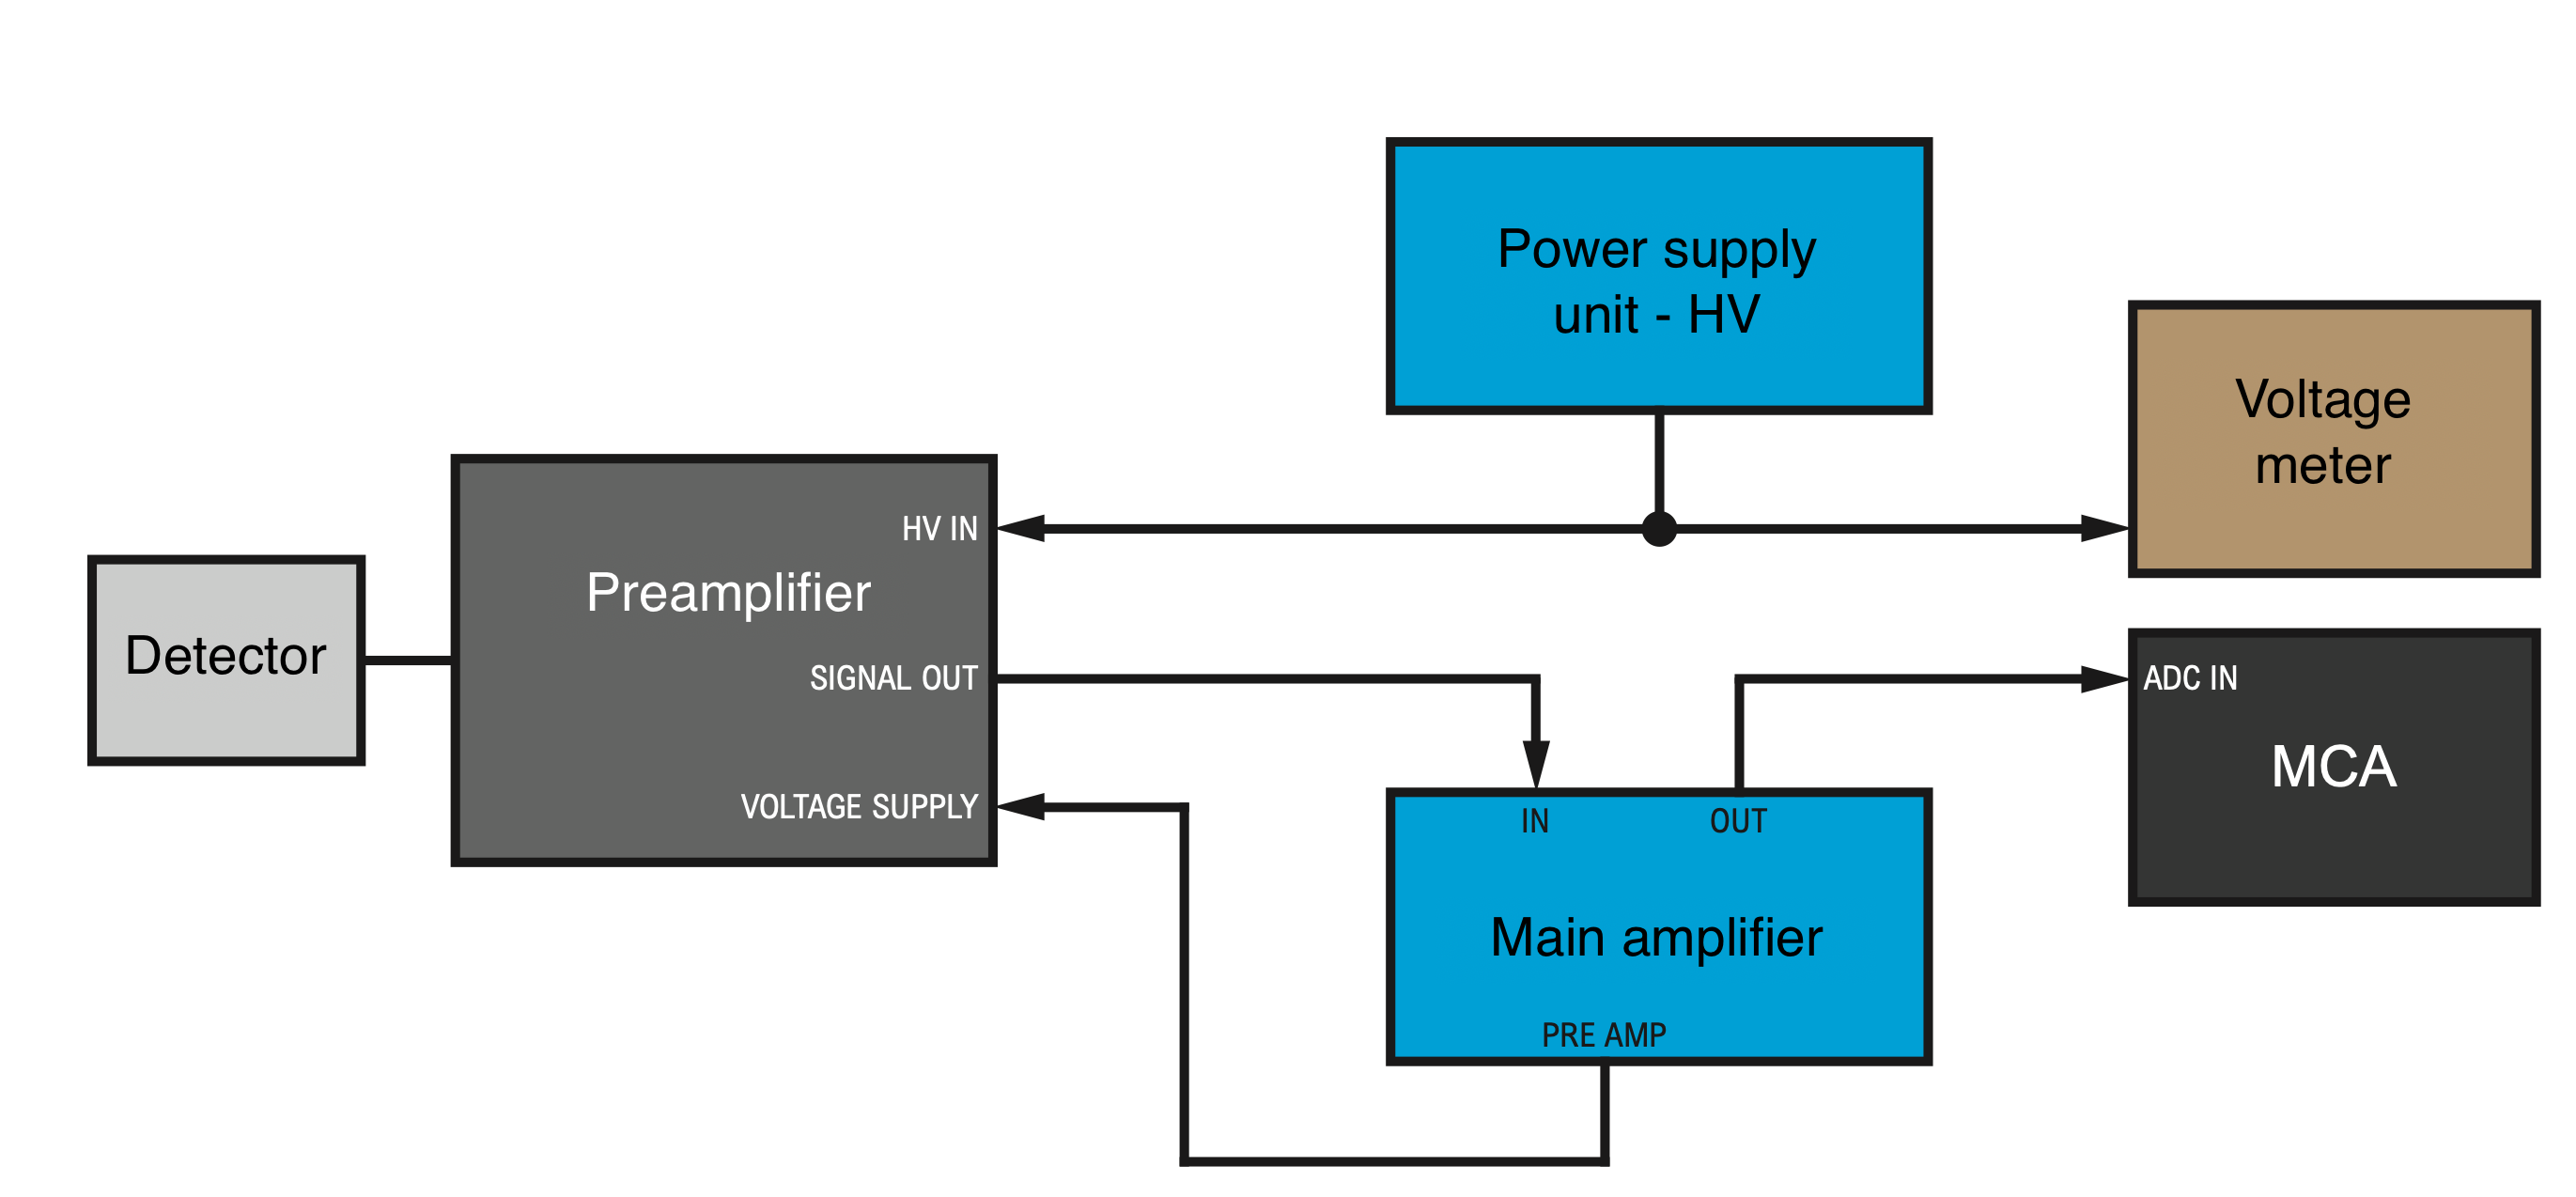
\includegraphics[width=\linewidth]{img/wiring.png}
	\caption{Schematics of the wiring of the experiment.}
	\label{fig:verkabelung}
\end{figure}

\begin{figure}
	\centering
	\subcaptionbox{View from the left. \label{fig:setup1}}[.49\linewidth]{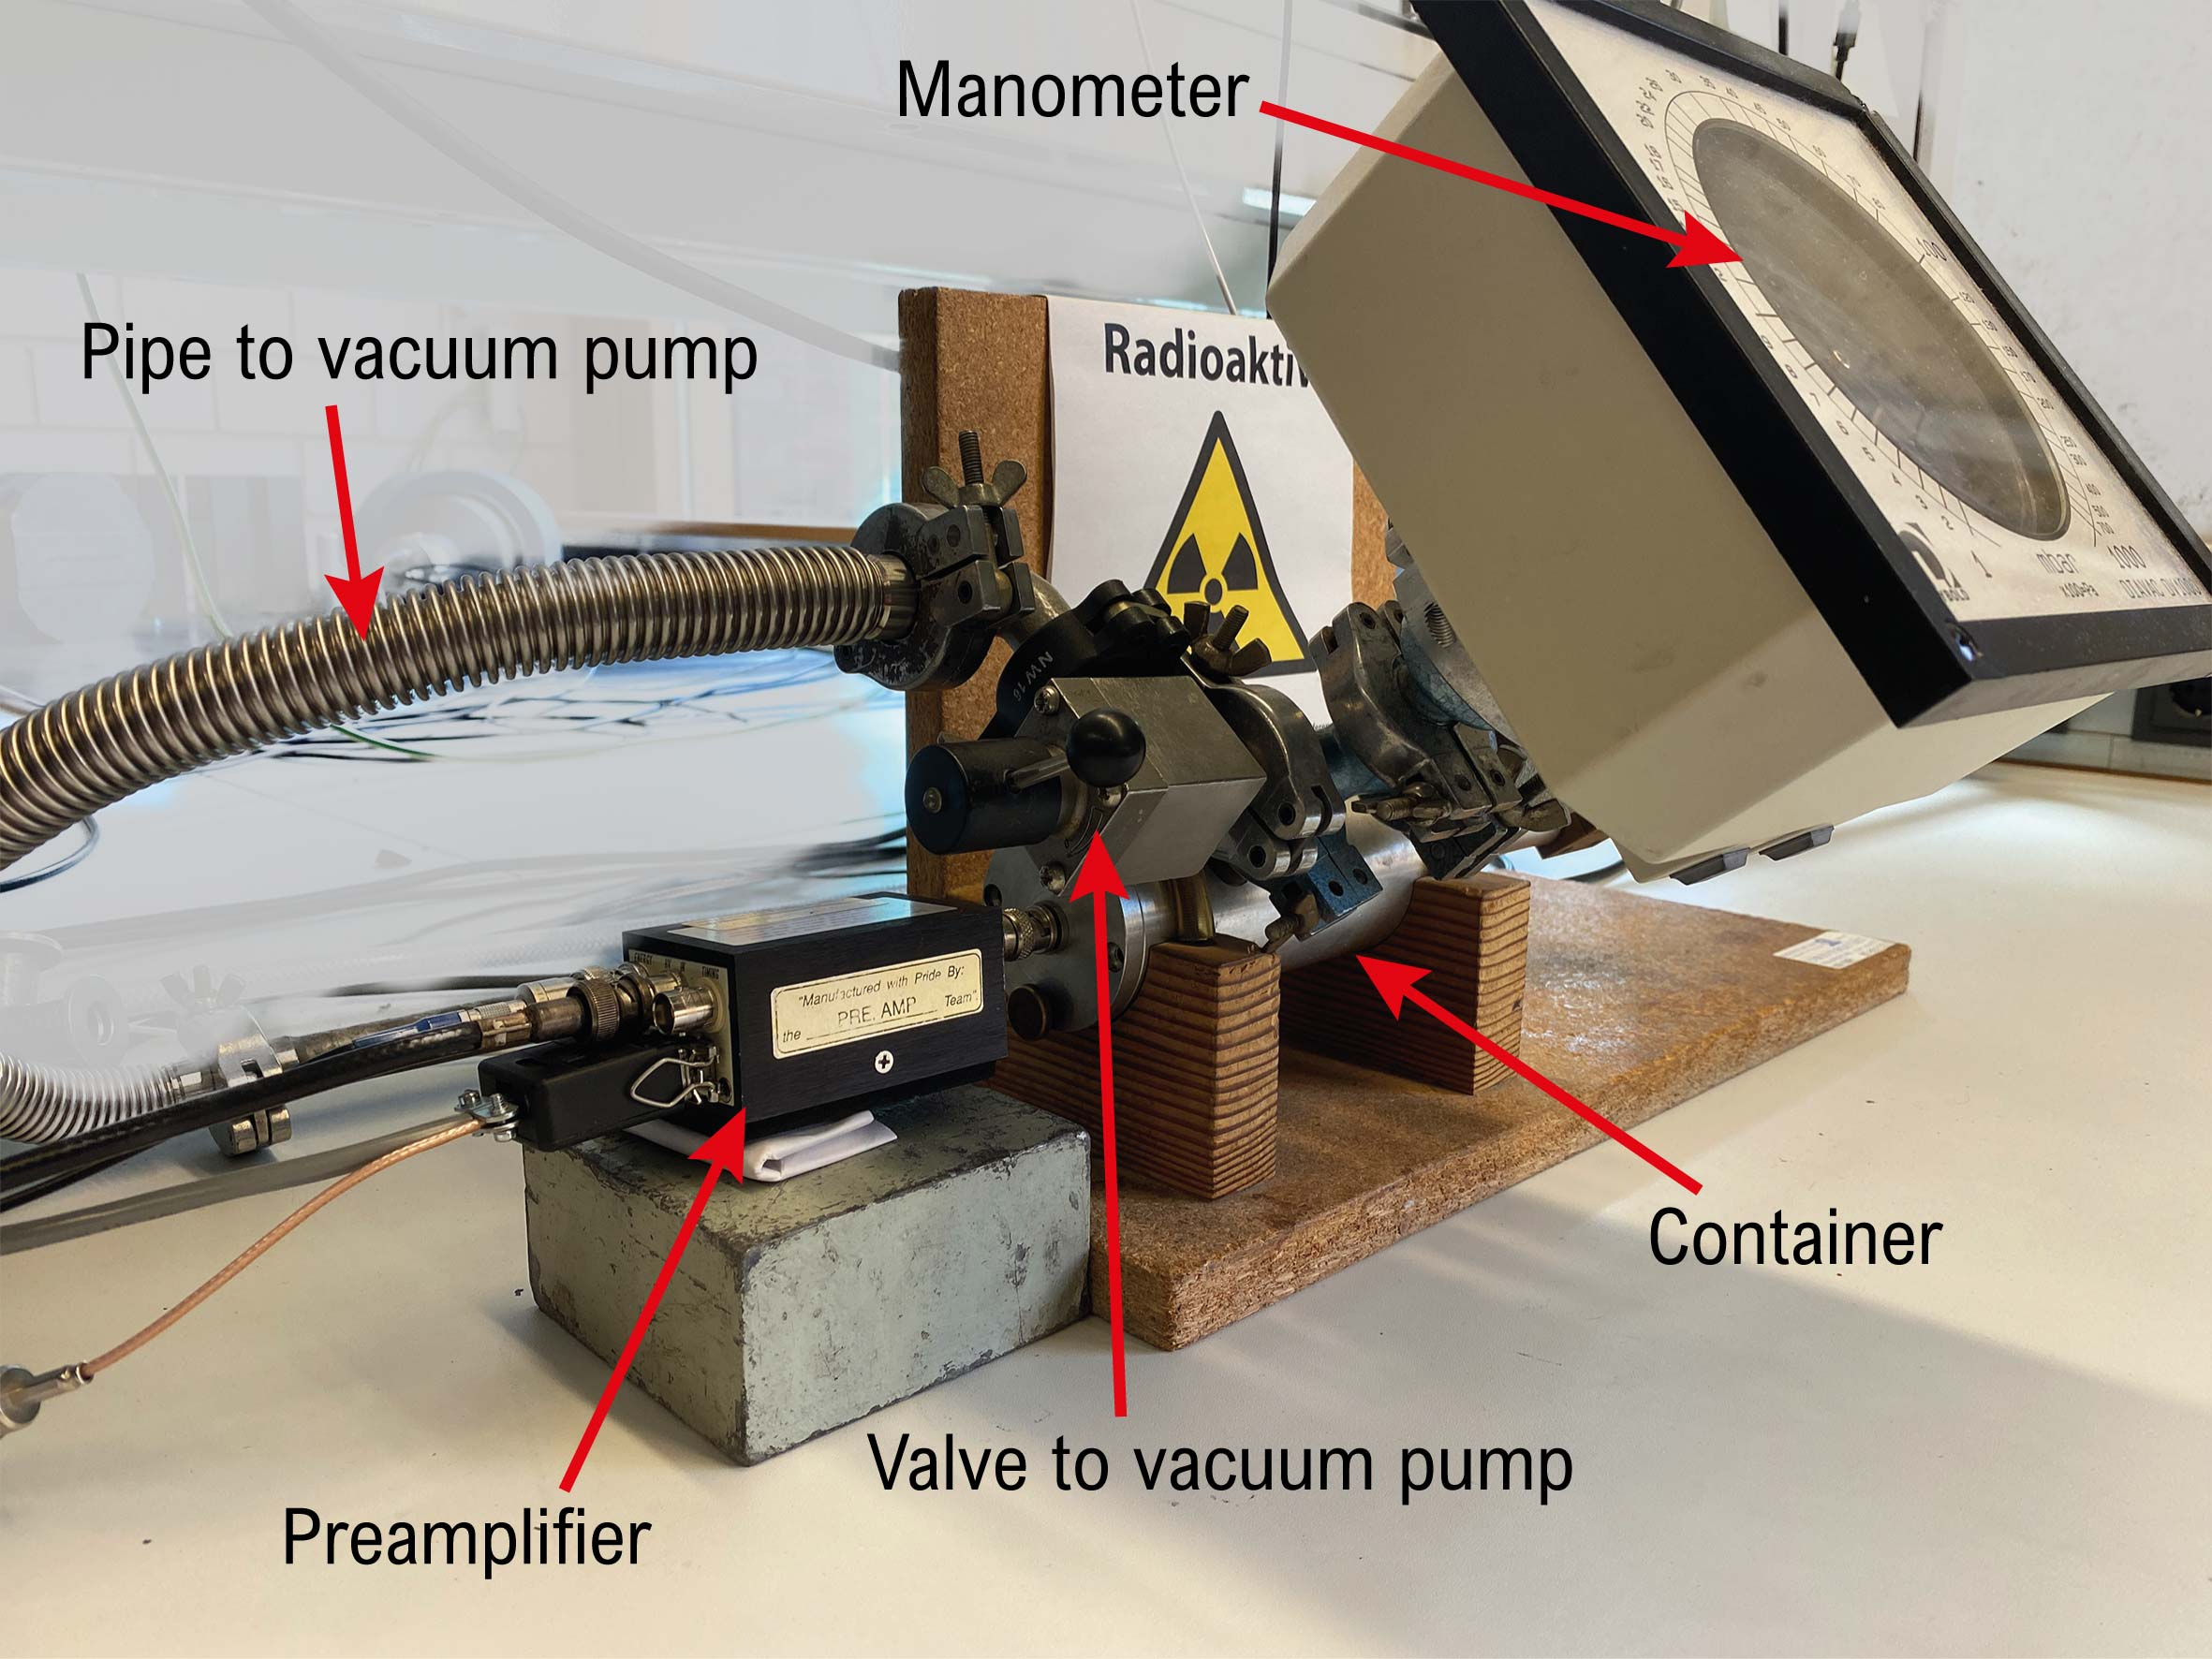
\includegraphics[width=\linewidth]{img/setup_1.jpg}}
	\subcaptionbox{View from the right. \label{fig:setup2}}[.49\linewidth]{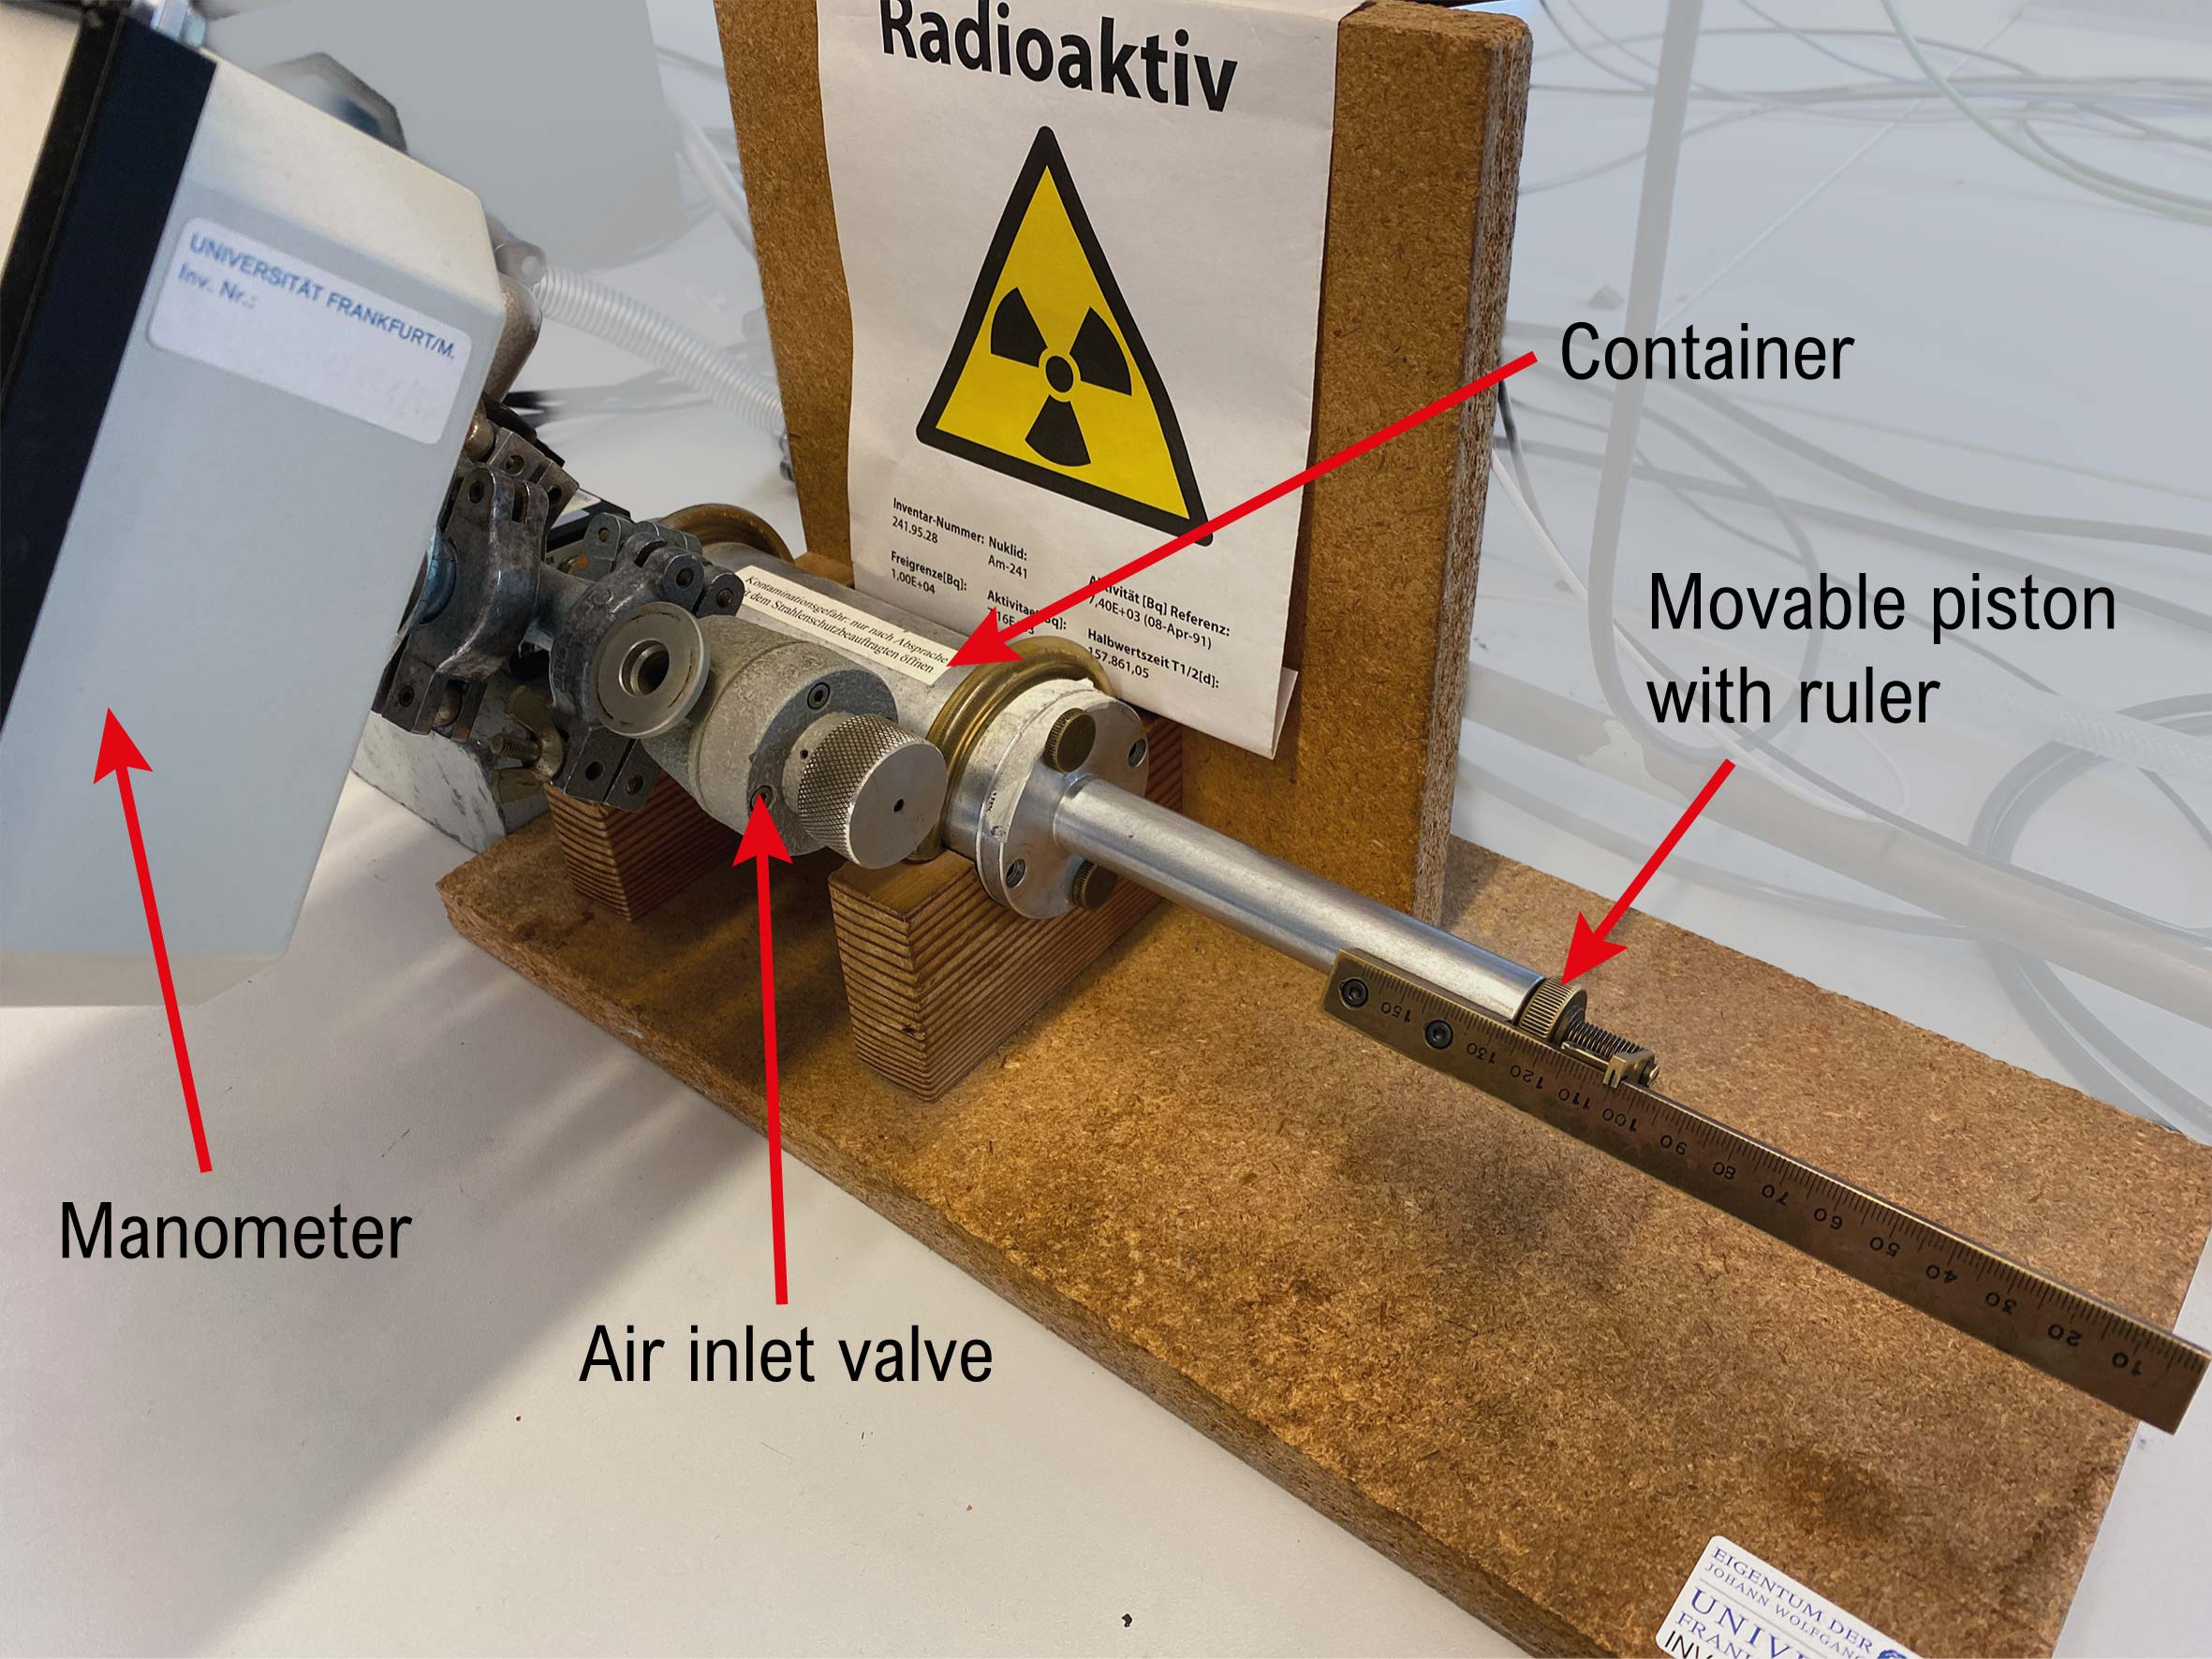
\includegraphics[width=\linewidth]{img/setup_2.jpg}}
	\caption{The experimental setup.}
	\label{fig:setup_}
\end{figure}
\begin{figure}
	\centering
	\subcaptionbox{The semiconductor detector. \label{fig:detektorfoto}}[.49\linewidth]
	{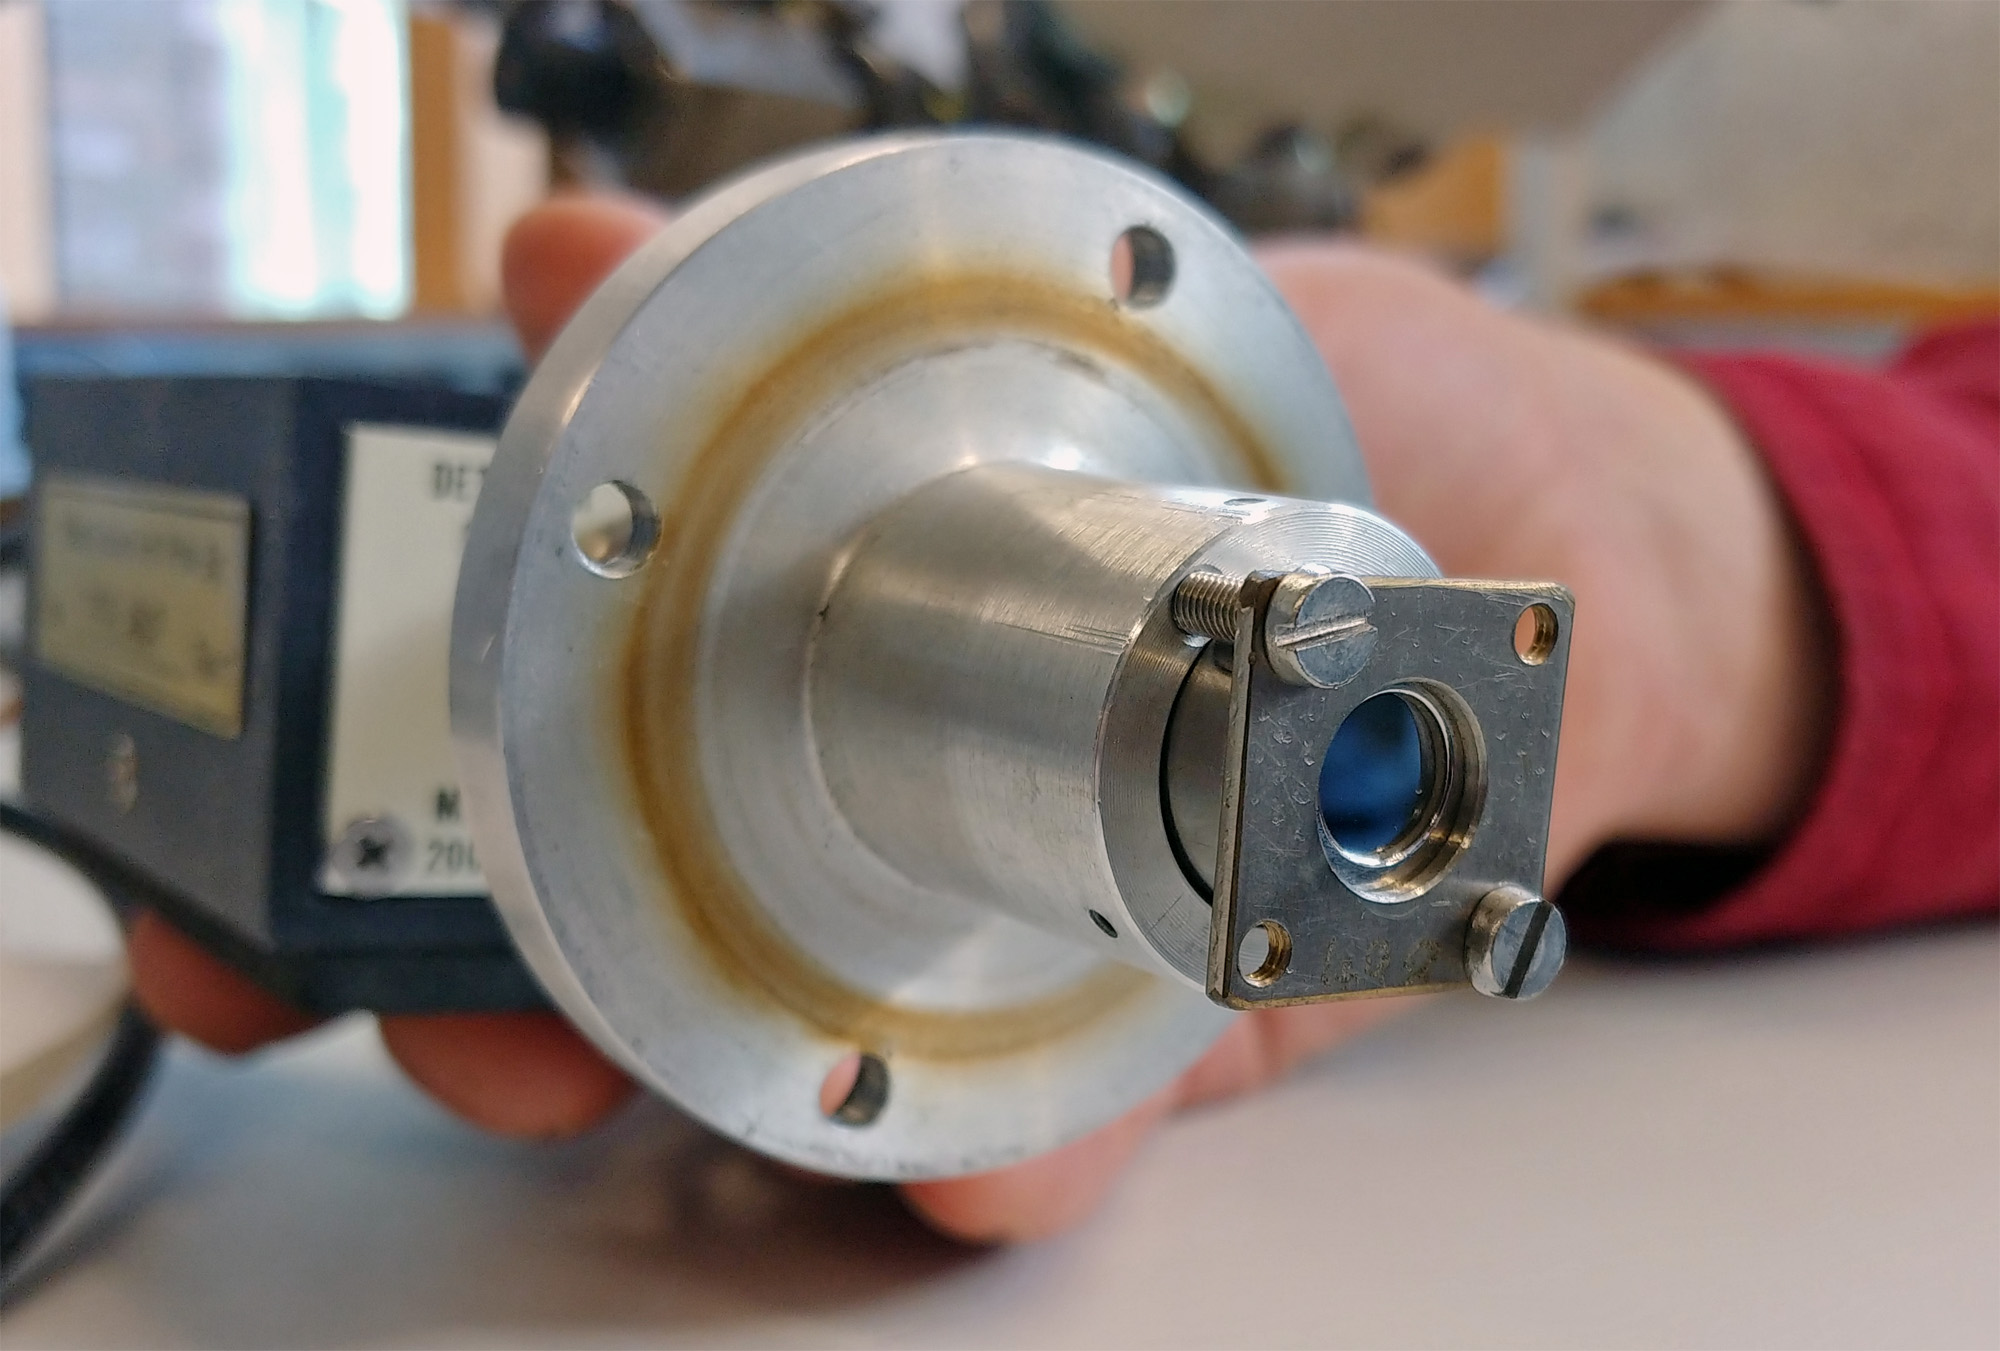
\includegraphics[width=\linewidth]{img/detektor_foto}}
	\subcaptionbox{The radiation source with golden surface. \label{fig:quellefoto}}[.49\linewidth]
	{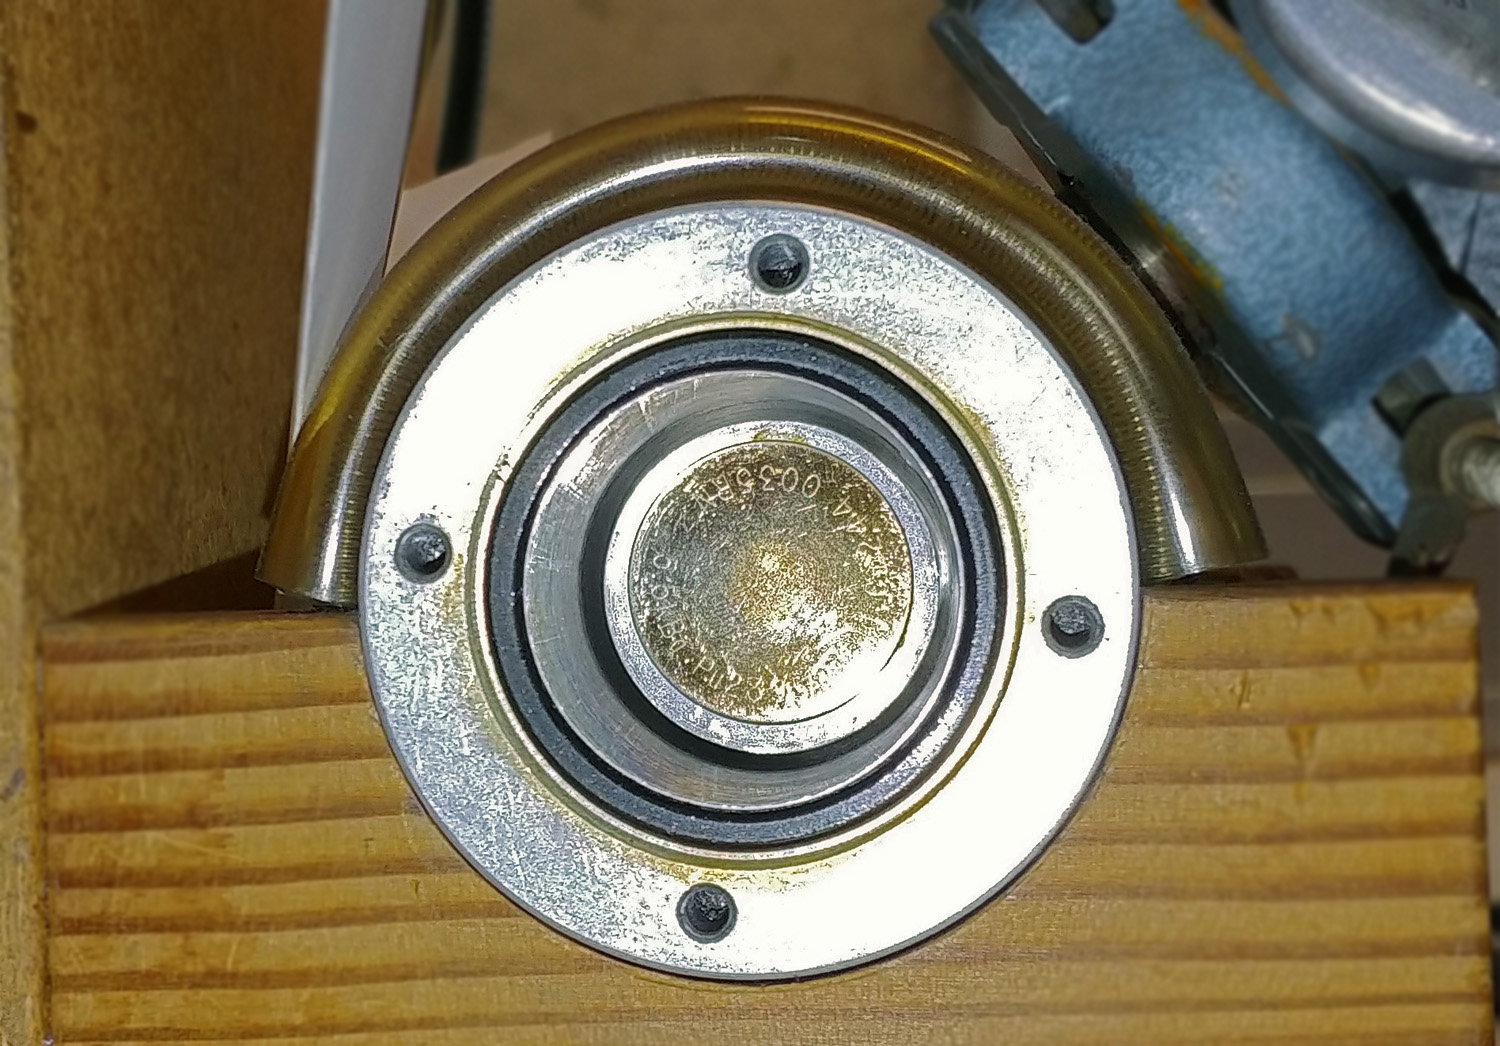
\includegraphics[width=\linewidth]{img/quelle_foto}}
	\caption{Interior views of the vacuum container.}
\end{figure}
\begin{figure}
	\centering
	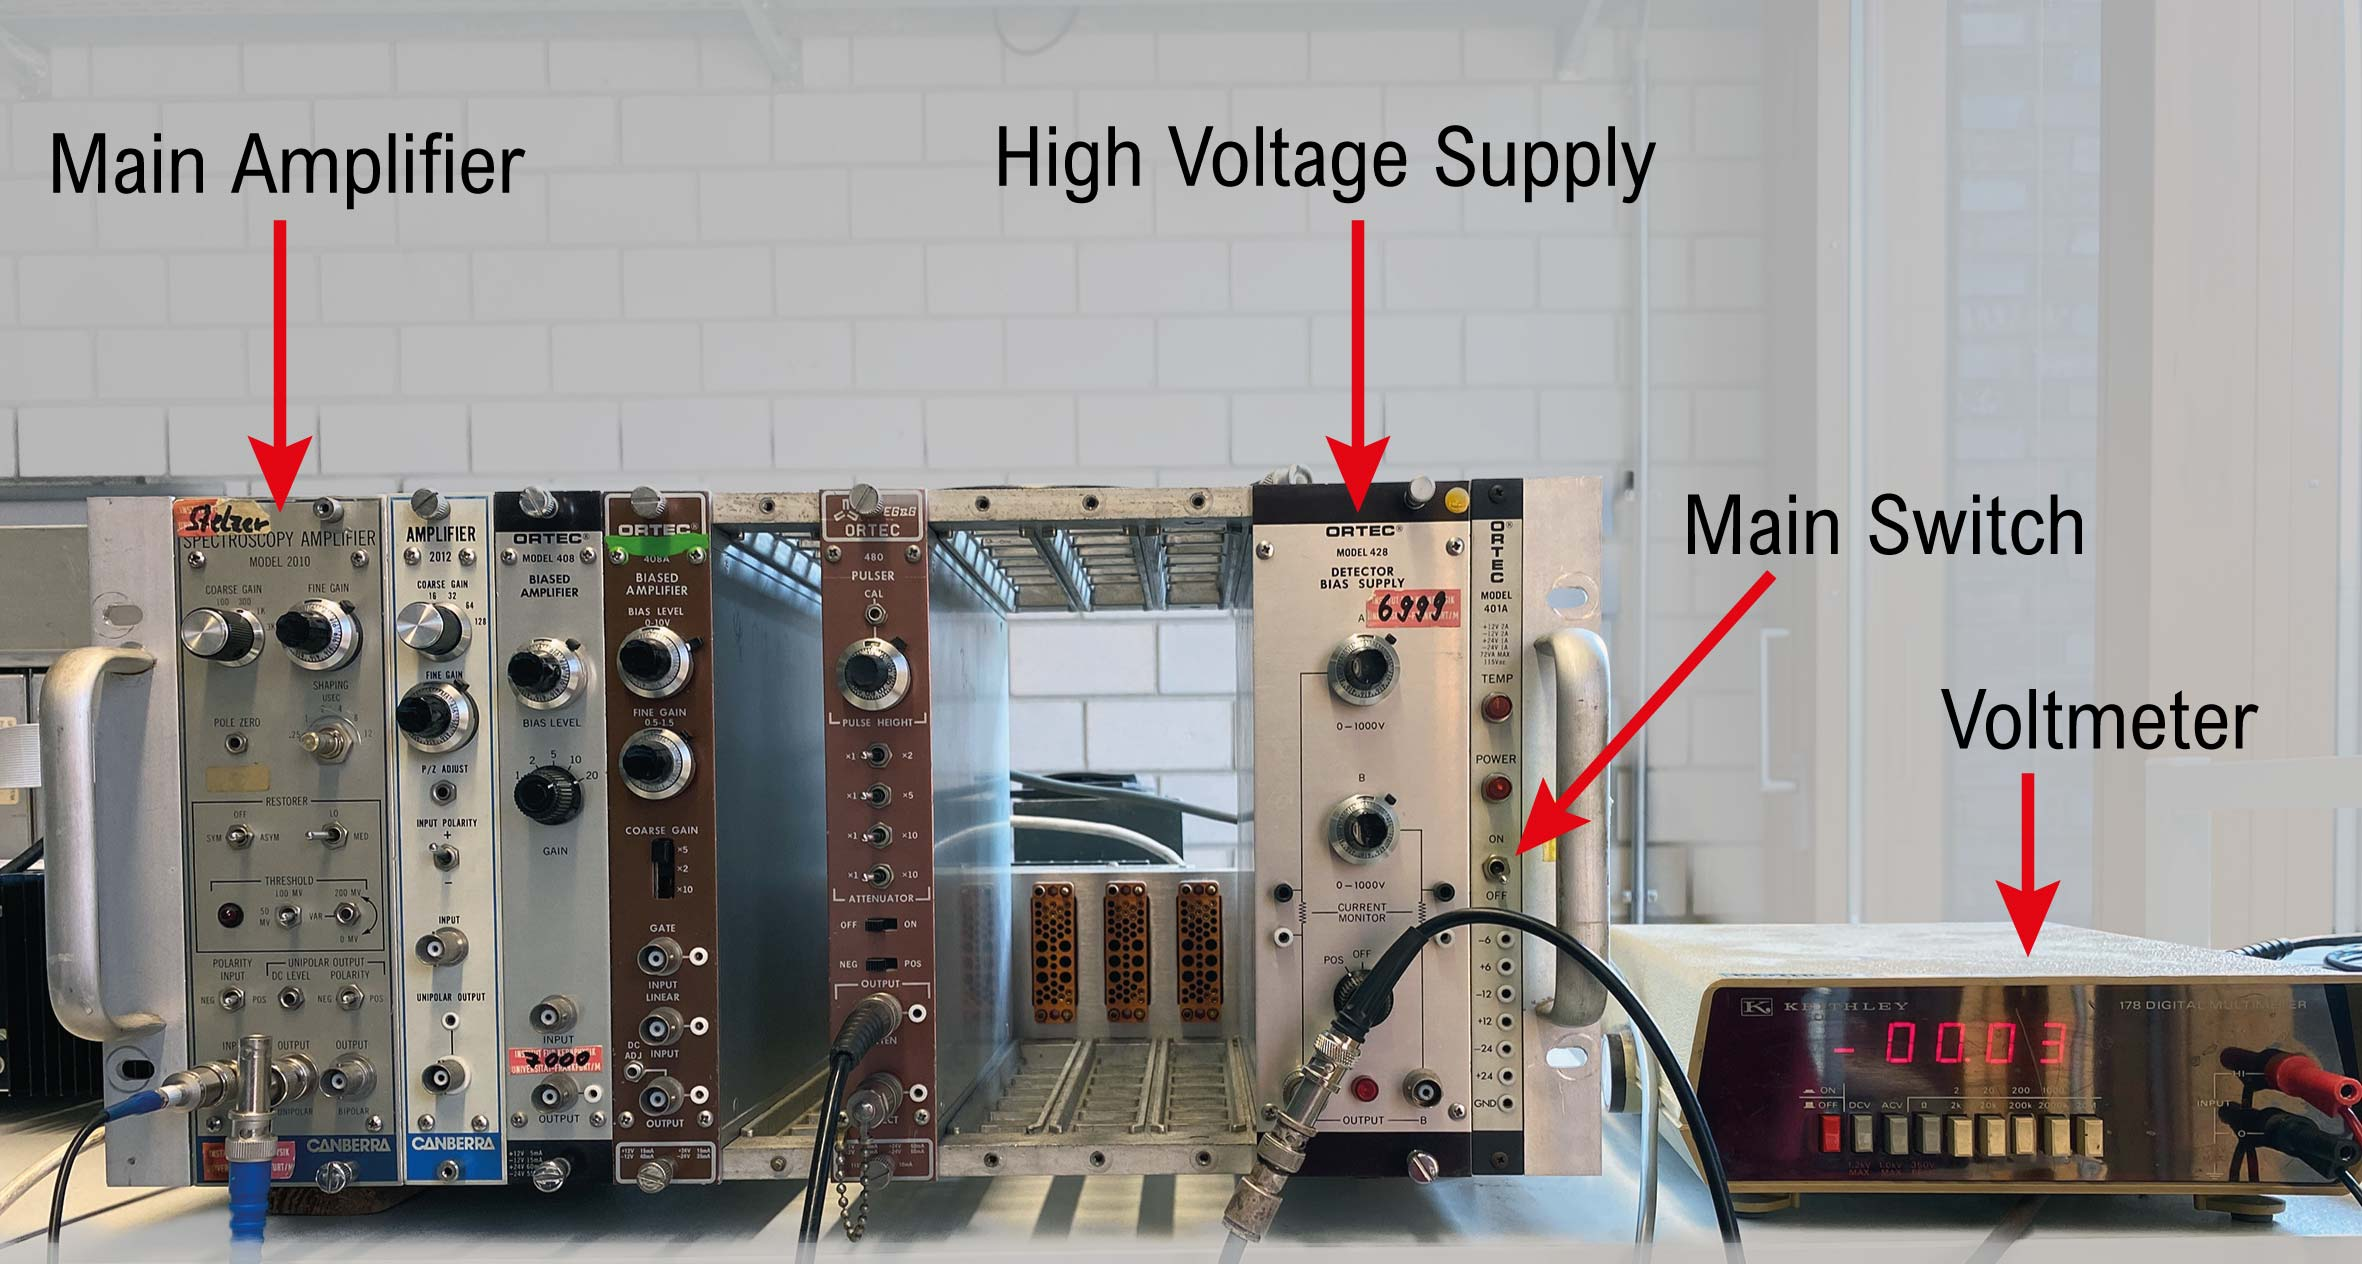
\includegraphics[width=0.75\linewidth]{img/setup_3.jpg}
	\caption{Electronics in the \enquote{Ortec-Crate}.}
	\label{fig:setup3}
\end{figure}
